\section{BC02 - Analyse exploratoire, descriptive et inférentielle de données}

\begin{frame}
    \centering
    \huge
    BC02 - Analyse exploratoire, descriptive et inférentielle de données
\end{frame}

% ===
% Présentation des ddatasets
% ===

\begin{frame}{Présentation des datasets}
	\small
	\begin{columns}[T]
		% ===
		% GUITARSET
		% ===
		\column{0.48\textwidth}
		
		\textbf{GuitarSet \cite{xi2018guitarset}} \quad \href{https://guitarset.weebly.com/}{\beamergotobutton{Dataset}}
		\begin{itemize}
			\item 360 extraits d'environs 30 s chacun.
			\item 6 guitaristes, 5 styles, 3 progressions, 2 tempi.
			\item Guitare acoustique et accordage standard.
			\item Captation hexaphonique et micro room.
			\item Audio WAV mono ou stéréo, 44100 Hz.
			\item Annotations temporelles au format JAMS.
			\item Licence Creative Commons Attribution 4.0 International.
		\end{itemize}
		
		% ===
		% IDMT
		% ===
		\column{0.48\textwidth}
		
		\textbf{IDMT-SMT-Guitar \cite{kehling2023idmt}} \quad \href{https://www.idmt.fraunhofer.de/en/publications/datasets/guitar.html}{\beamergotobutton{Dataset}}
		\begin{itemize}
			\item 7 guitares en accordage standard.
			\item Différents micros et configurations.
			\item Audio WAV mono, 44100 Hz.
			\item Annotations au format XML.
			\item Techniques de jeu.
			\item Licence Creative Commons Attribution \textbf{Non Commercial No Derivatives} 4.0 International.
		\end{itemize}
	\end{columns}
	
	\vspace{0.2cm}
	
	\begin{block}{Conclusion}
		Les deux datasets sont complémentaires. GuitarSet contient des annotations et contextes musicaux riches et IDMT-SMT-Guitar apporte une diversité instrumentale et des techniques de jeu.
	\end{block}
\end{frame}

% ===
% Analyse GuitarSet
% ===

\begin{frame}{Analyse du dataset GuitarSet - Métadonnées}
	\begin{table}
		\centering
		\small
		\begin{tabular}{l l l c l l l c}
			\hline
			guitarist\_id & title & style & tempo & scale & mode & playing\_version & duration \\
			\hline
			0 & 00\_BN1-129-Eb\_comp & BN1 & 129 & Eb & major & comp & 22.32 \\
			\hline
		\end{tabular}
	\end{table}
	
	\begin{columns}[T]
		\column{0.6\textwidth}
		
		\begin{figure}
			\centering
			
\includegraphics[height=4cm]{figures/BC02/metadata_categorical_variables_distributions.png}
		\end{figure}
		
		\small
		Bien que les styles musicaux soient équirépartis, le dataset présente un léger déséquilibre des classes sur les gammes et les modes.
		
		\column{0.39\textwidth}
		
		\begin{figure}
			\centering
			
\includegraphics[height=4cm]{figures/BC02/metadata_categorical_variables_correlation_matrix.png}
		\end{figure}
		
		\small
		Chaque style est associé à un mode.
		Chaque gamme semble préférentiellement associée à un style
		musical ou à un mode.
	\end{columns}
\end{frame}

\begin{frame}{Analyse du dataset GuitarSet - Métadonnées}
	\vspace{-0.4cm}
	
	\begin{columns}[T]
		\column{0.49\textwidth}
		
		\begin{figure}
			\centering
			
\includegraphics[width=\textwidth]{figures/BC02/metadata_numerical_variables_distributions.png}
		\end{figure}
		
		\small
		Les conditions sont favorables à une analyse de corrélation : absence d'outliers, distribution relativement symétrique, dispersions non pathologiques et kurtosis raisonnables.
		
		\column{0.49\textwidth}
		
		\begin{figure}
			\centering
			
\includegraphics[width=\textwidth]{figures/BC02/metadata_numerical_variables_correlation_matrix.png}
		\end{figure}
		
		\small
		Il semble que plus le tempo d'un morceau est rapide, plus il est court et réciproquement. Cette relation est raisonnablement linéaire.
	\end{columns}
\end{frame}

\begin{frame}{Analyse du dataset GuitarSet - Métadonnées}
	\vspace{-0.4cm}
	
	\begin{columns}[T]
		\column{0.42\textwidth}
		
		\begin{figure}
			\centering
			
\includegraphics[height=3.6cm]{figures/BC02/metadata_categorical_and_numerical_variables_correlation_matrix.png}
		\end{figure}
		
		\small
		Les styles musicaux semblent préférentiellement associés à des tempi et des durées.
		
		\column{0.57\textwidth}
		
		\begin{figure}
			\centering
			
\includegraphics[height=3.6cm]{figures/BC02/metadata_categorical_and_numerical_variables_boxplots.png}
		\end{figure}
		
		\small
		Les styles présentent des profils rythmiques distincts et influencent la durée des extraits. Les étendues des tempi et des durées varient selon la gamme.
	\end{columns}
	
	\begin{block}{\small Conclusion}
		\small
		L'analyse des métadonnées montre des corrélations entre \textbf{style}, \textbf{gamme}, \textbf{tempo} et \textbf{durée}. Ces dépendances caractérisent la distribution du dataset et peuvent influencer l'apprentissage du modèle.
	\end{block}
\end{frame}

\begin{frame}{Analyse du dataset GuitarSet - Annotations}
	\begin{table}
		\centering
		\small
		\begin{tabular}{l c c c c}
			\hline
			title & data\_source & time & duration & value \\
			\hline
			00\_BN1-129-Eb\_comp & 0 & 7.457274 & 0.464399 & 44.018917 \\
			\hline
		\end{tabular}
	\end{table}
	
	\begin{columns}[T]
		\column{0.44\textwidth}
		
		\vspace{0.2cm}
		
		\small
		\textbf{Hauteur de notes par corde}
		\begin{table}
			\centering
			\tiny
			\begin{tabular}{l c c c c}
				\hline
				string & min & theoretical\_min & max & theoretical\_max \\
				\hline
				E2 & 39.79 & 40 & 54.01 & 59 \\
				A2 & 44.68 & 45 & 58.06 & 64 \\
				D3 & 49.75 & 50 & 69.10 & 69 \\
				G3 & 54.63 & 55 & 73.09 & 74 \\
				B3 & 58.60 & 59 & 78.39 & 78 \\
				E4 & 63.58 & 64 & 80.98 & 83 \\
				\hline
			\end{tabular}
		\end{table}
		
		\small
		Pas d'anomalie détectée : les intervalles des hauteurs de notes réelles et théoriques coïncident.
		
		\column{0.52\textwidth}
		
		\begin{figure}
			\centering
			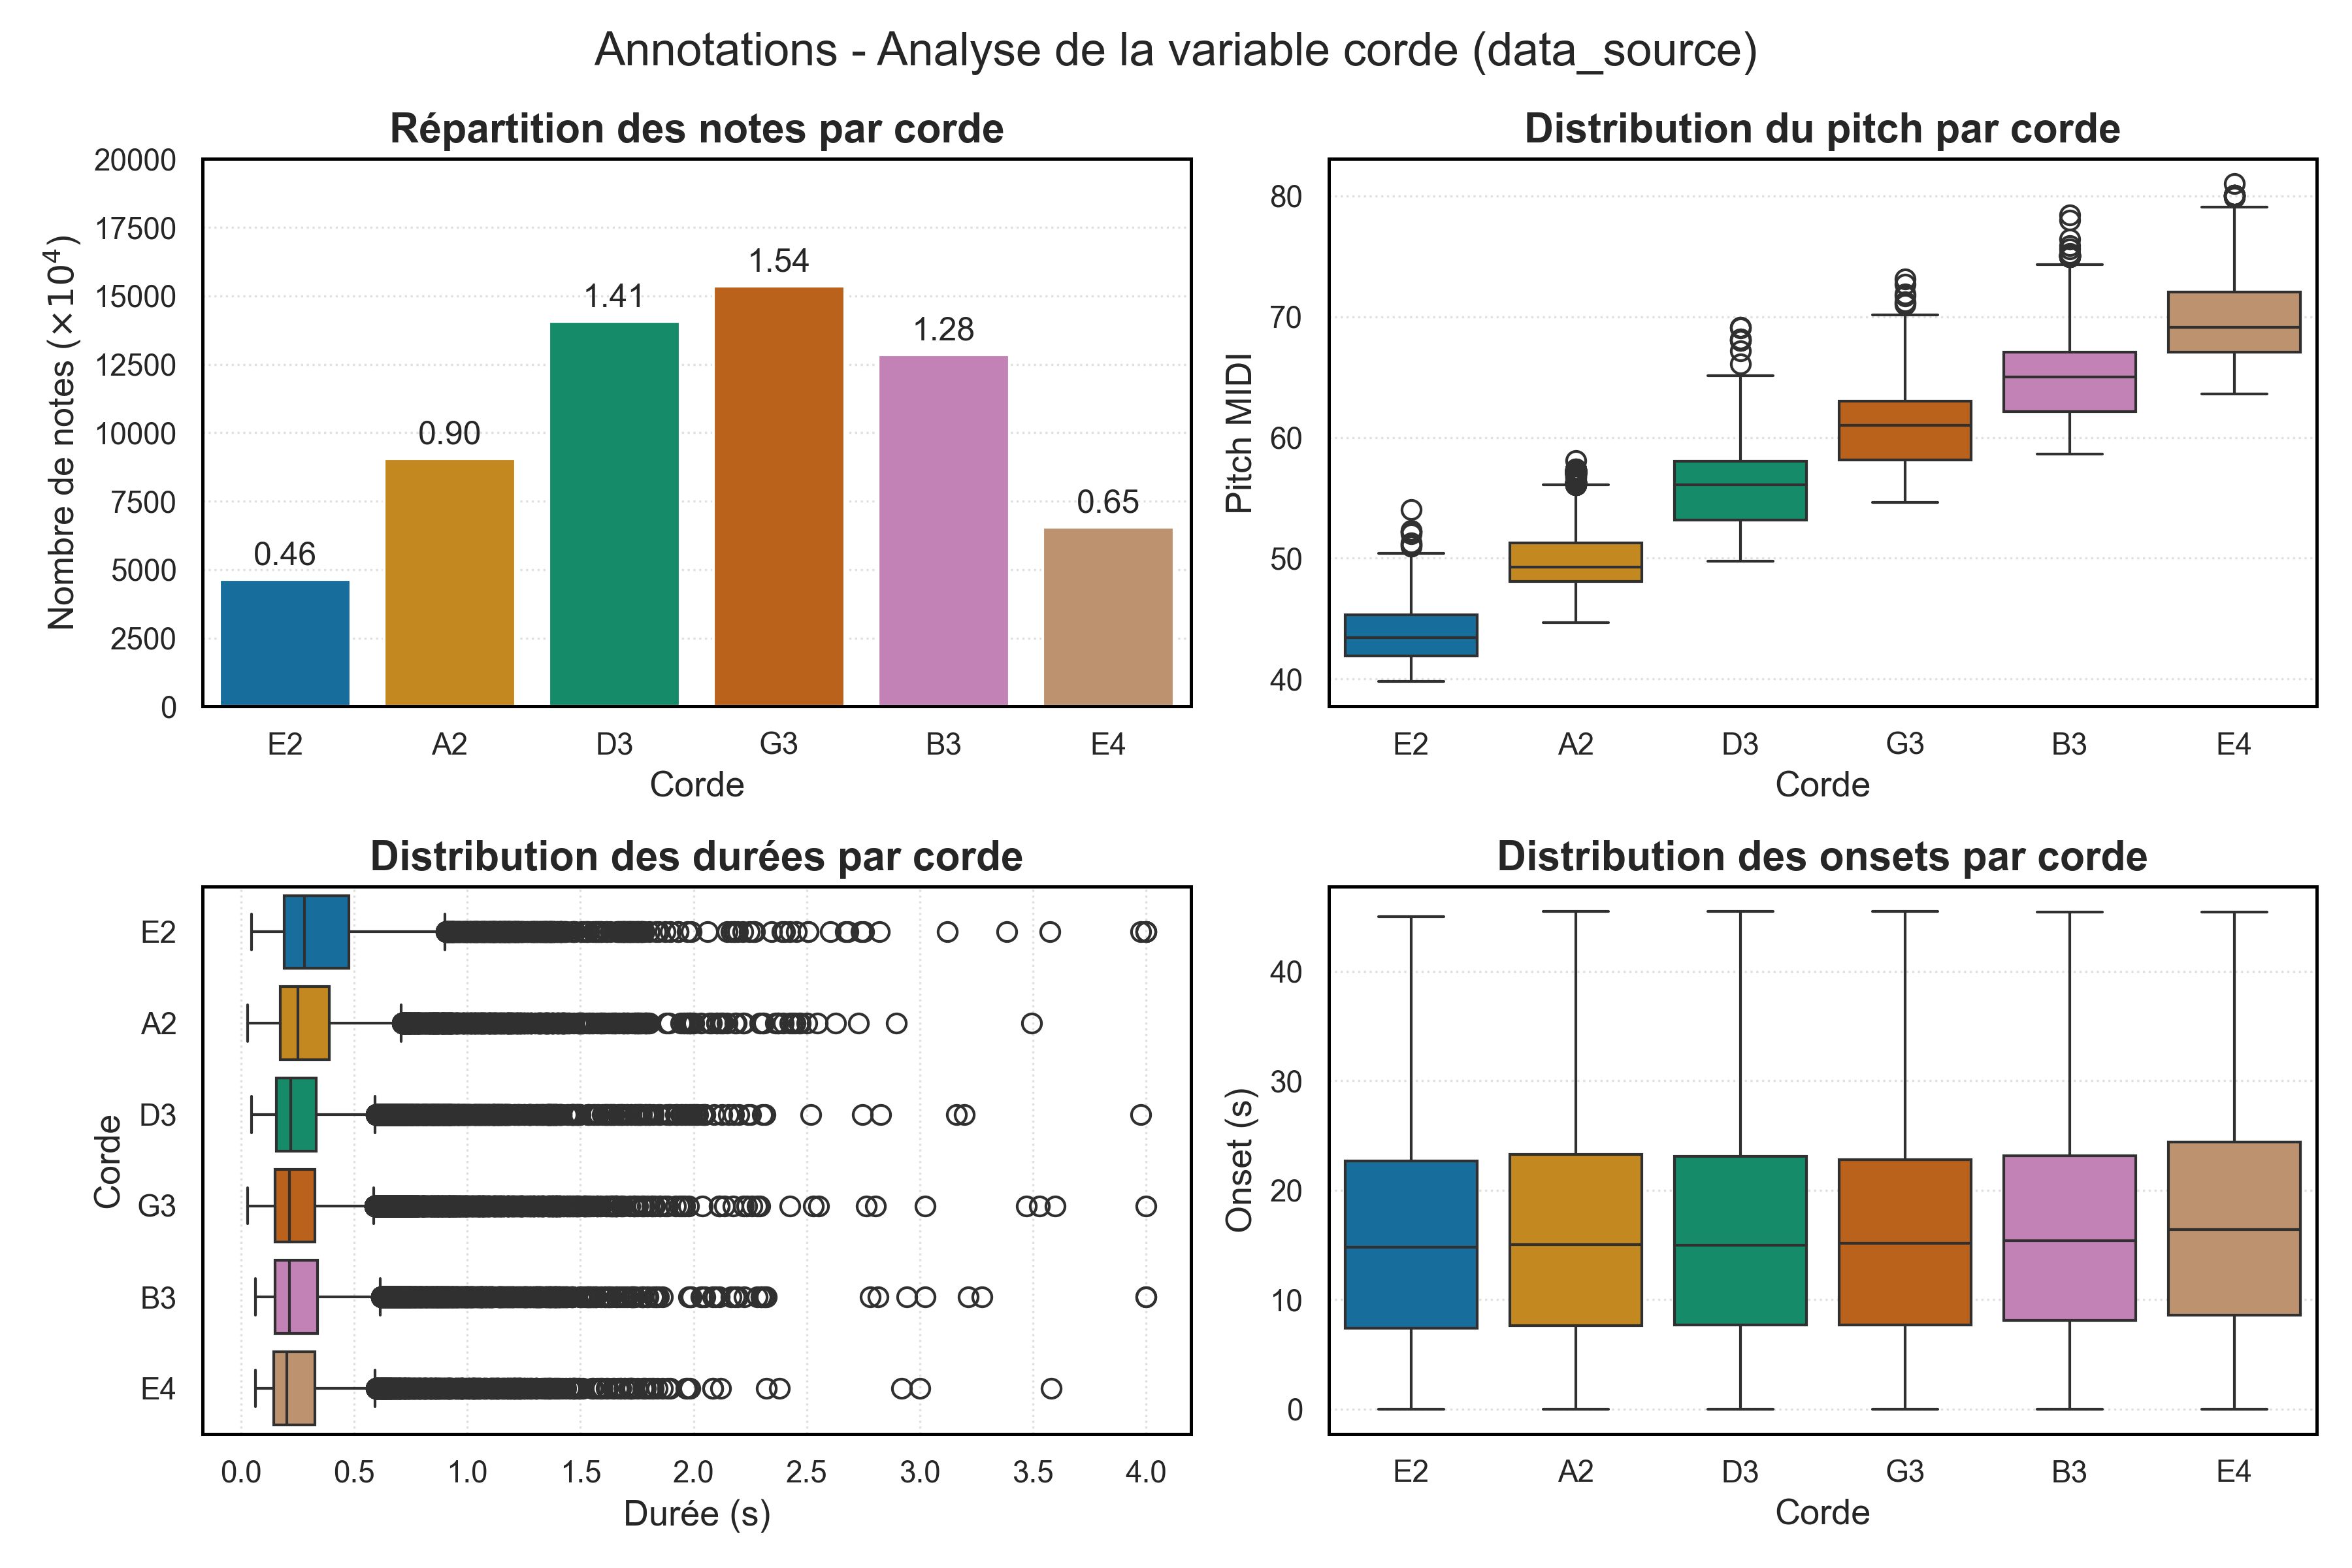
\includegraphics[height=3.6cm]{figures/BC02/annotation_data_source_analysis.png}
		\end{figure}
		
		\small
		Les annotations semblent cohérentes avec la physique de l'instrument.
		La sous représentation des notes graves devrait être balancée par leurs durées. En revanche, la sous représentation des notes aiguës couplée à leur durée courte laisse présager des difficultés de transcription pour ces notes.
	\end{columns}
\end{frame}

%\begin{frame}{Analyse du dataset GuitarSet - Annotations}
%	\begin{columns}[T]
%		\column{0.49\textwidth}
%		\vspace{-0.4cm}
%		
%		\begin{figure}
%			\centering
%			
\includegraphics[width=\textwidth]{figures/BC02/annotation_numerical_variables_distributions.png}
%		\end{figure}
%		
%		\column{0.49\textwidth}
%		
%		\small
%		Activations sans biais.
%		Distribution des durées fortement asymétrique avec de nombreuses valeurs extrêmes plausibles.
%		La distribution des hauteurs de notes offre une bonne représentation du registre de la guitare.
%		
%		\begin{figure}
%			\centering
%			
\includegraphics[width=\textwidth]{figures/BC02/annotation_numerical_variables_correlations.png}
%		\end{figure}
%		
%		\small
%		Hauteur de note et corde pincée sont fortement corrélées. Corrélation non parfaite dû au chevauchement des notes. On observe que plus la note est aiguë, moins elle dure.
%	\end{columns}
%\end{frame}

\begin{frame}{Analyse du dataset GuitarSet - Polyphonie et qualité audio}
	
	
	\vspace{0.2cm}
	
	
	\begin{columns}[T]
		\column{0.49\textwidth}
		
		\small
		\textbf{Activations simultanées}\\
		En considérant que des activations ayant au plus 20ms d'écart sont des notes activées simultanées, on peut estimer la polyphonie du dataset.
		\begin{itemize}
			\item En moyenne, 1,67 ($\pm 1,11$) notes activées simultanément.
			\item Au moins 25\% d'intervalle ou d'accords.
			\item Au maximum, 6 notes actives simultanément, ce qui correspond à la physique de l'instrument. 
		\end{itemize}
		
		\column{0.49\textwidth}
		
		
		\small
		\textbf{Qualité Audio}
		\begin{figure}
			\centering
			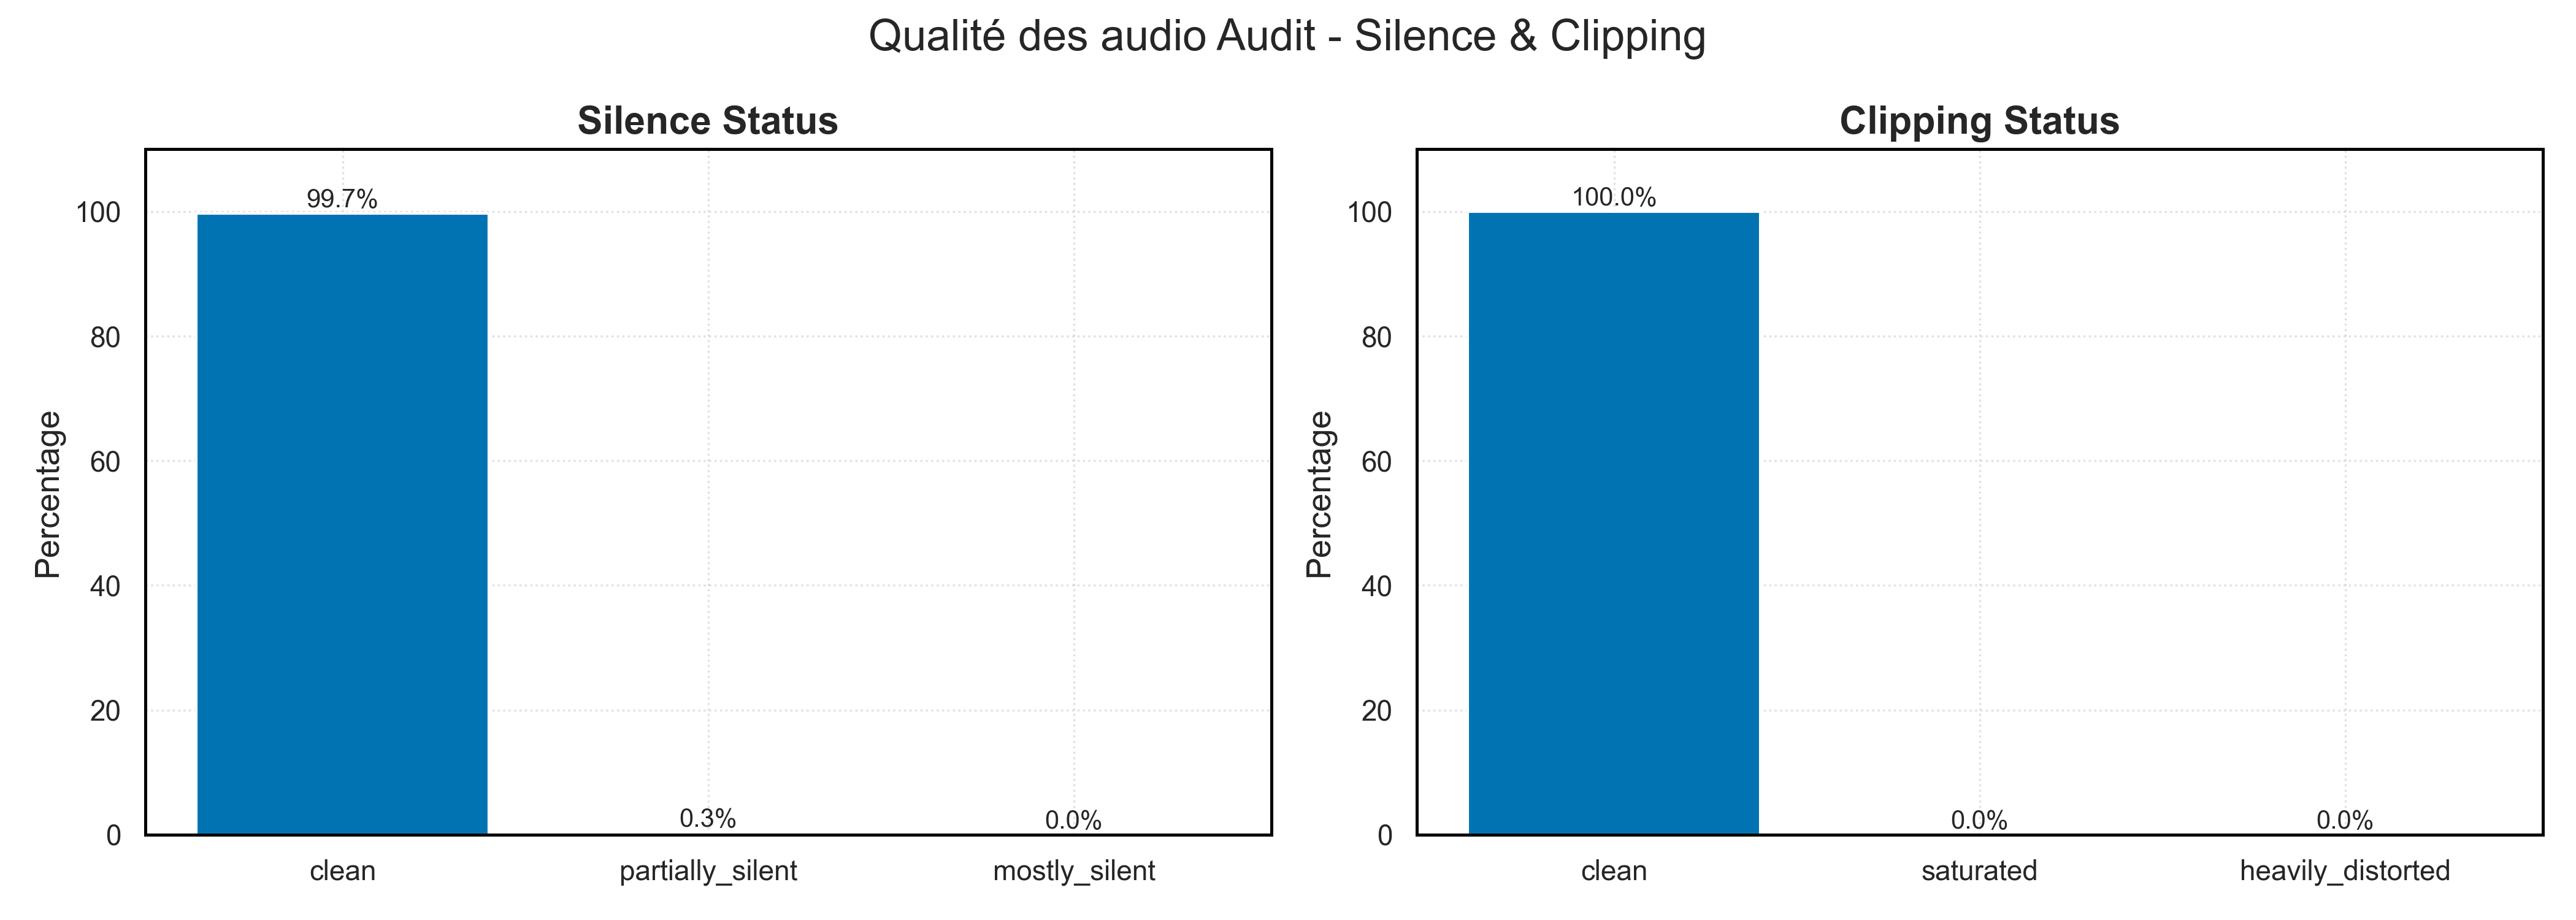
\includegraphics[width=\textwidth]{figures/BC02/audio_silence_clipping.png}
		\end{figure}
		
		\small
		Les audios sont propres, peu de silence et pas d'écrêtage.
	\end{columns}
	
	\begin{block}{\small Conclusion}
		\small
		Dataset riche mais partiellement contraint. Bonne base pour apprentissage supervisé. IDMT-SMT-Guitar constitue un complément intéressant.
	\end{block}
	
%	\small
%	\textbf{Chevauchement des notes}
%	\begin{columns}[T]
%		\column{0.49\textwidth}
%		\begin{figure}
%			\centering
%			
\includegraphics[width=\textwidth]{figures/BC02/piano_roll.png}
%		\end{figure}
%		
%		\column{0.49\textwidth}
%		
%		\begin{figure}
%			\centering
%			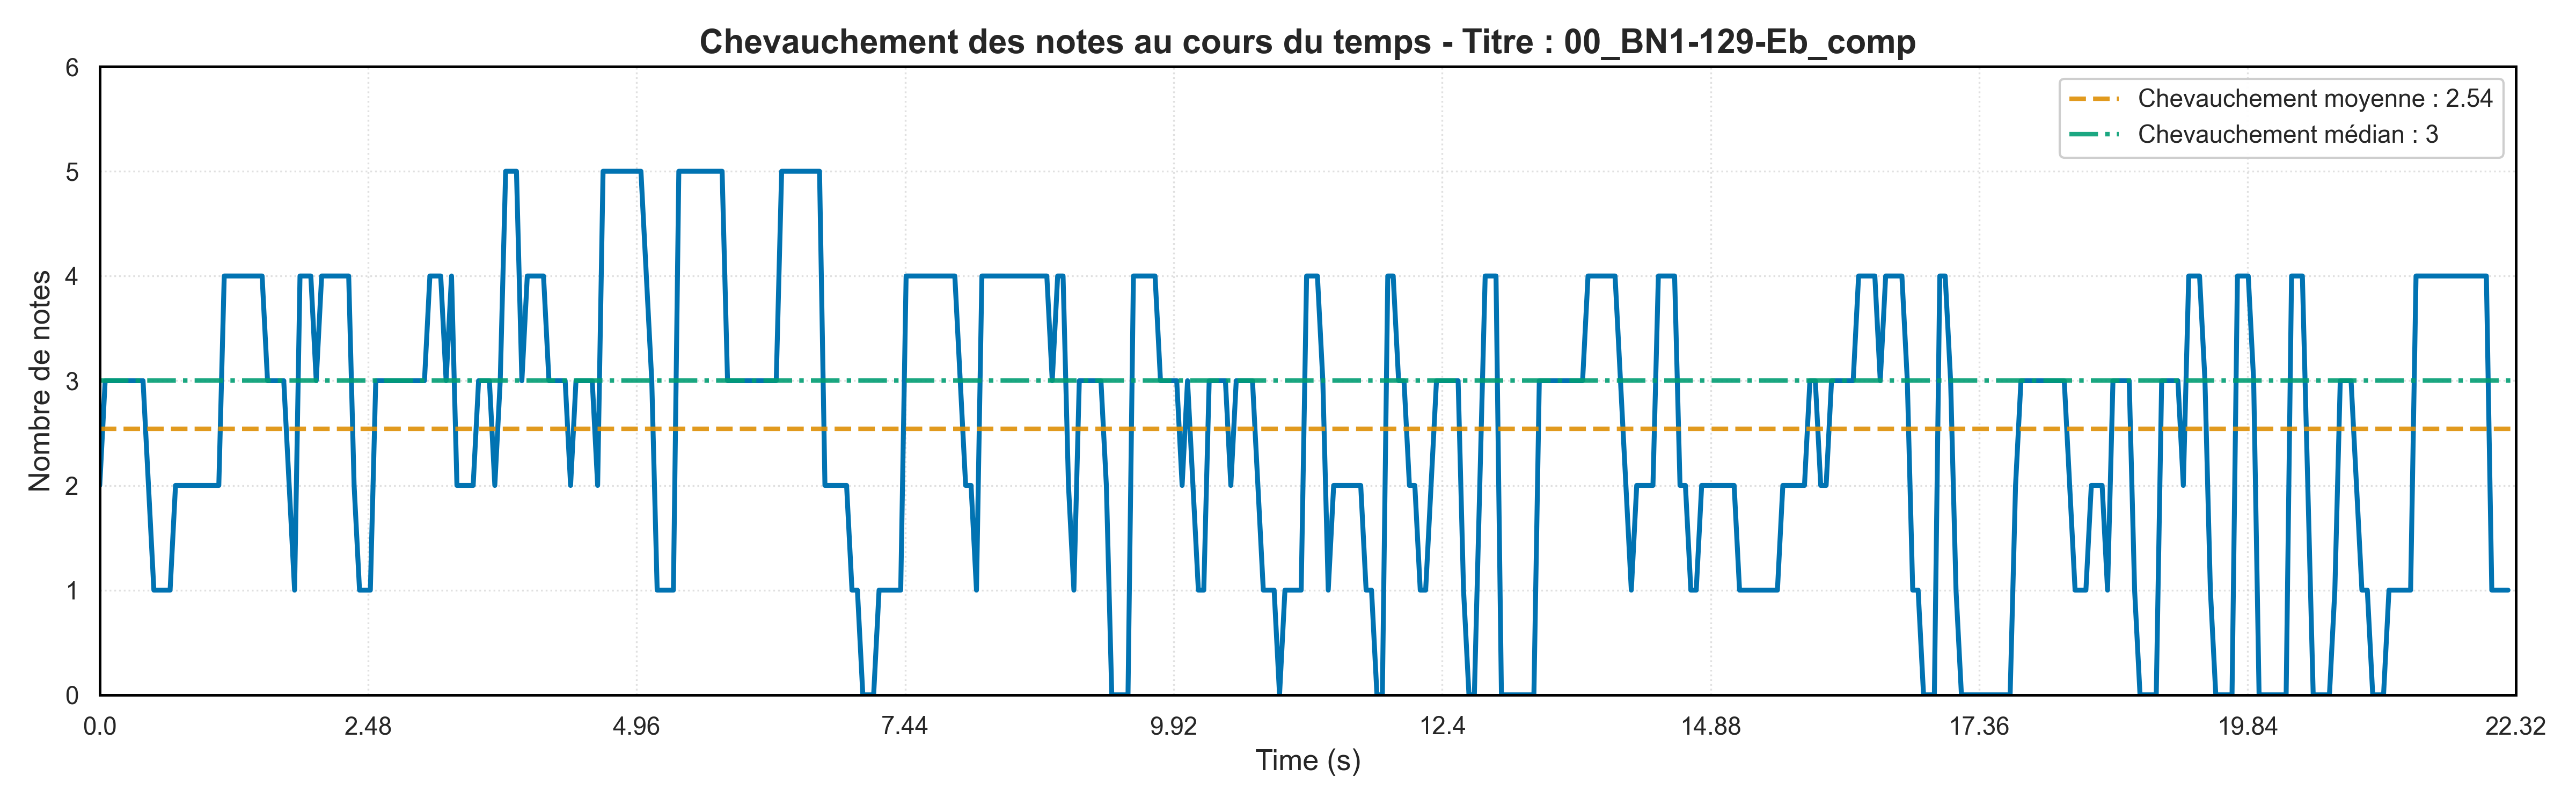
\includegraphics[width=\textwidth]{figures/BC02/overlapping.png}
%		\end{figure}
%	\end{columns}
%	
%	\small
%	Pour le titre 00\_BN1-129-Eb\_comp, on observe de nombreux chevauchements de notes. En moyenne, 2.54 chevauchement de notes.
\end{frame}

%\begin{frame}{Analyse du dataset GuitarSet - Audio}
%	\small
%	\textbf{Transformée Q constante}
%	\begin{columns}[T]
%		\column{0.49\textwidth}
%		\begin{figure}
%			\centering
%			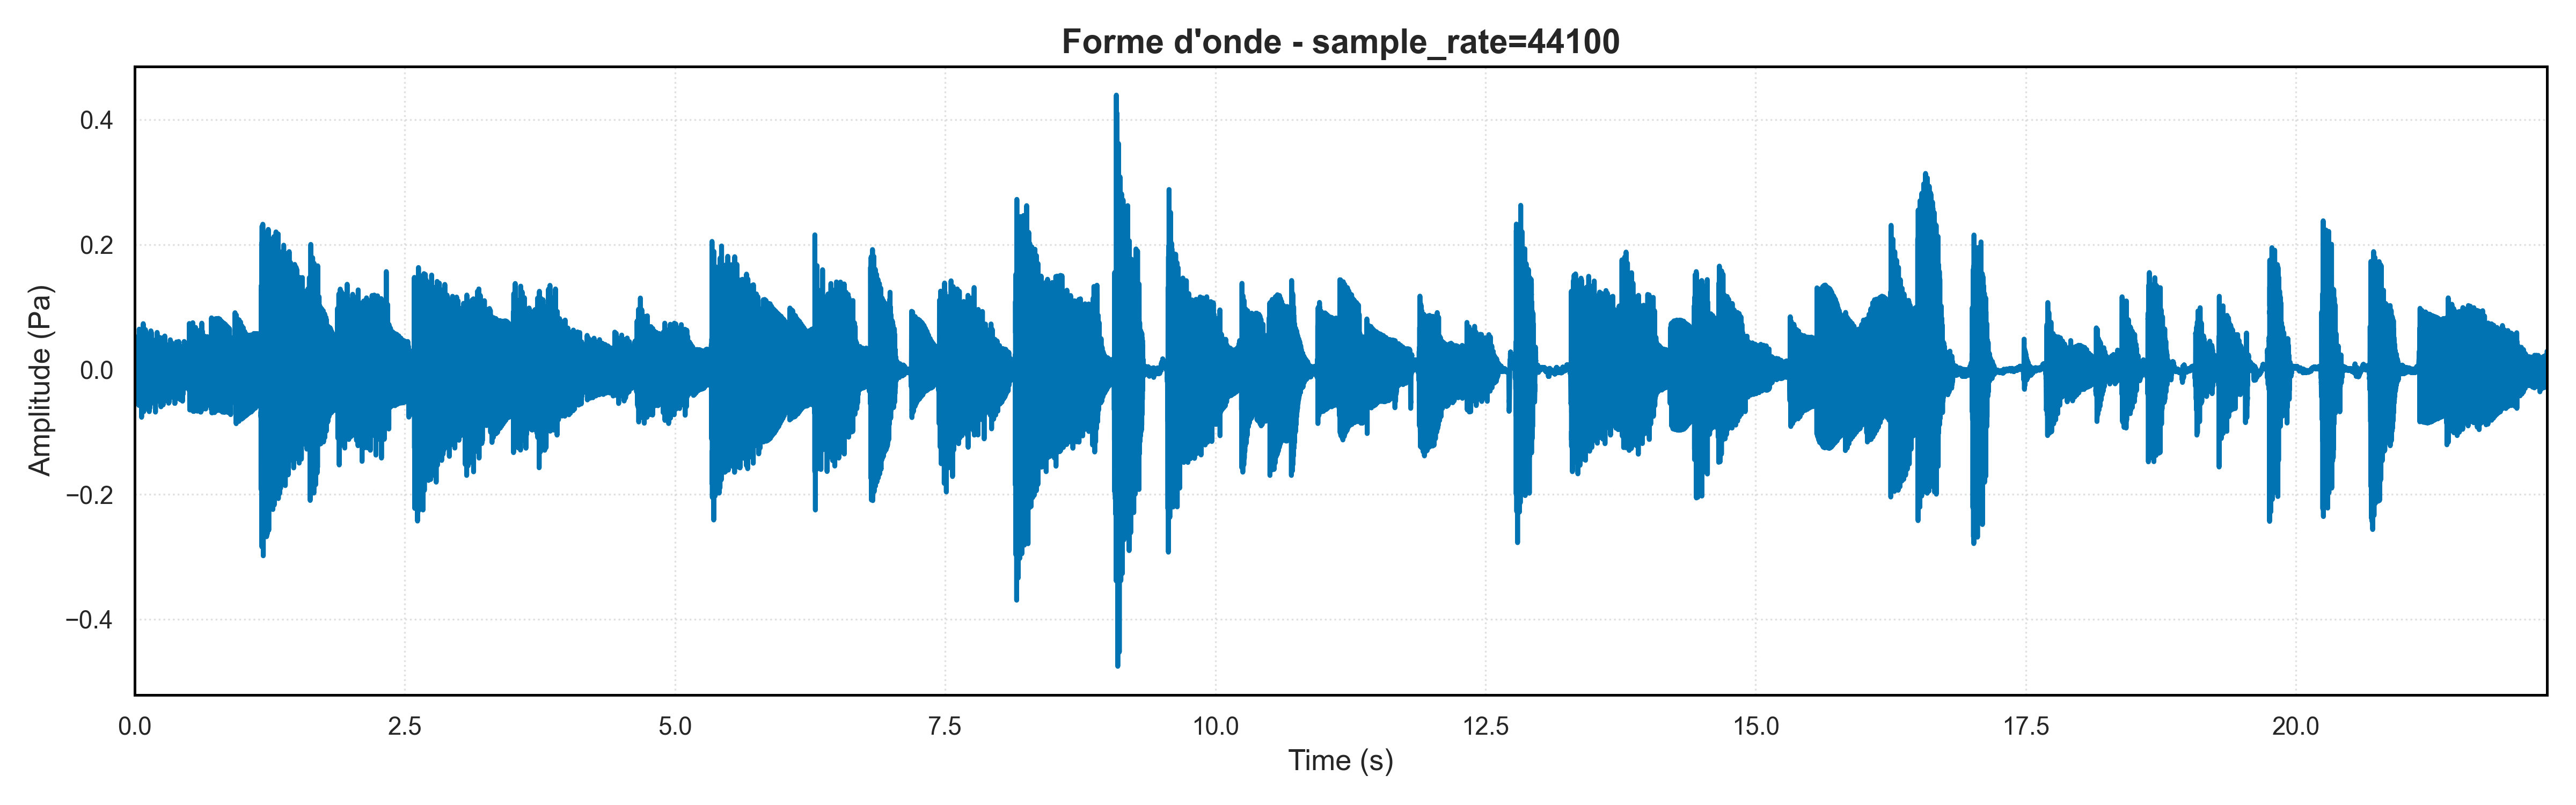
\includegraphics[height=2cm]{figures/BC02/waveform.png}
%		\end{figure}
%		
%		\begin{figure}
%		\centering
%		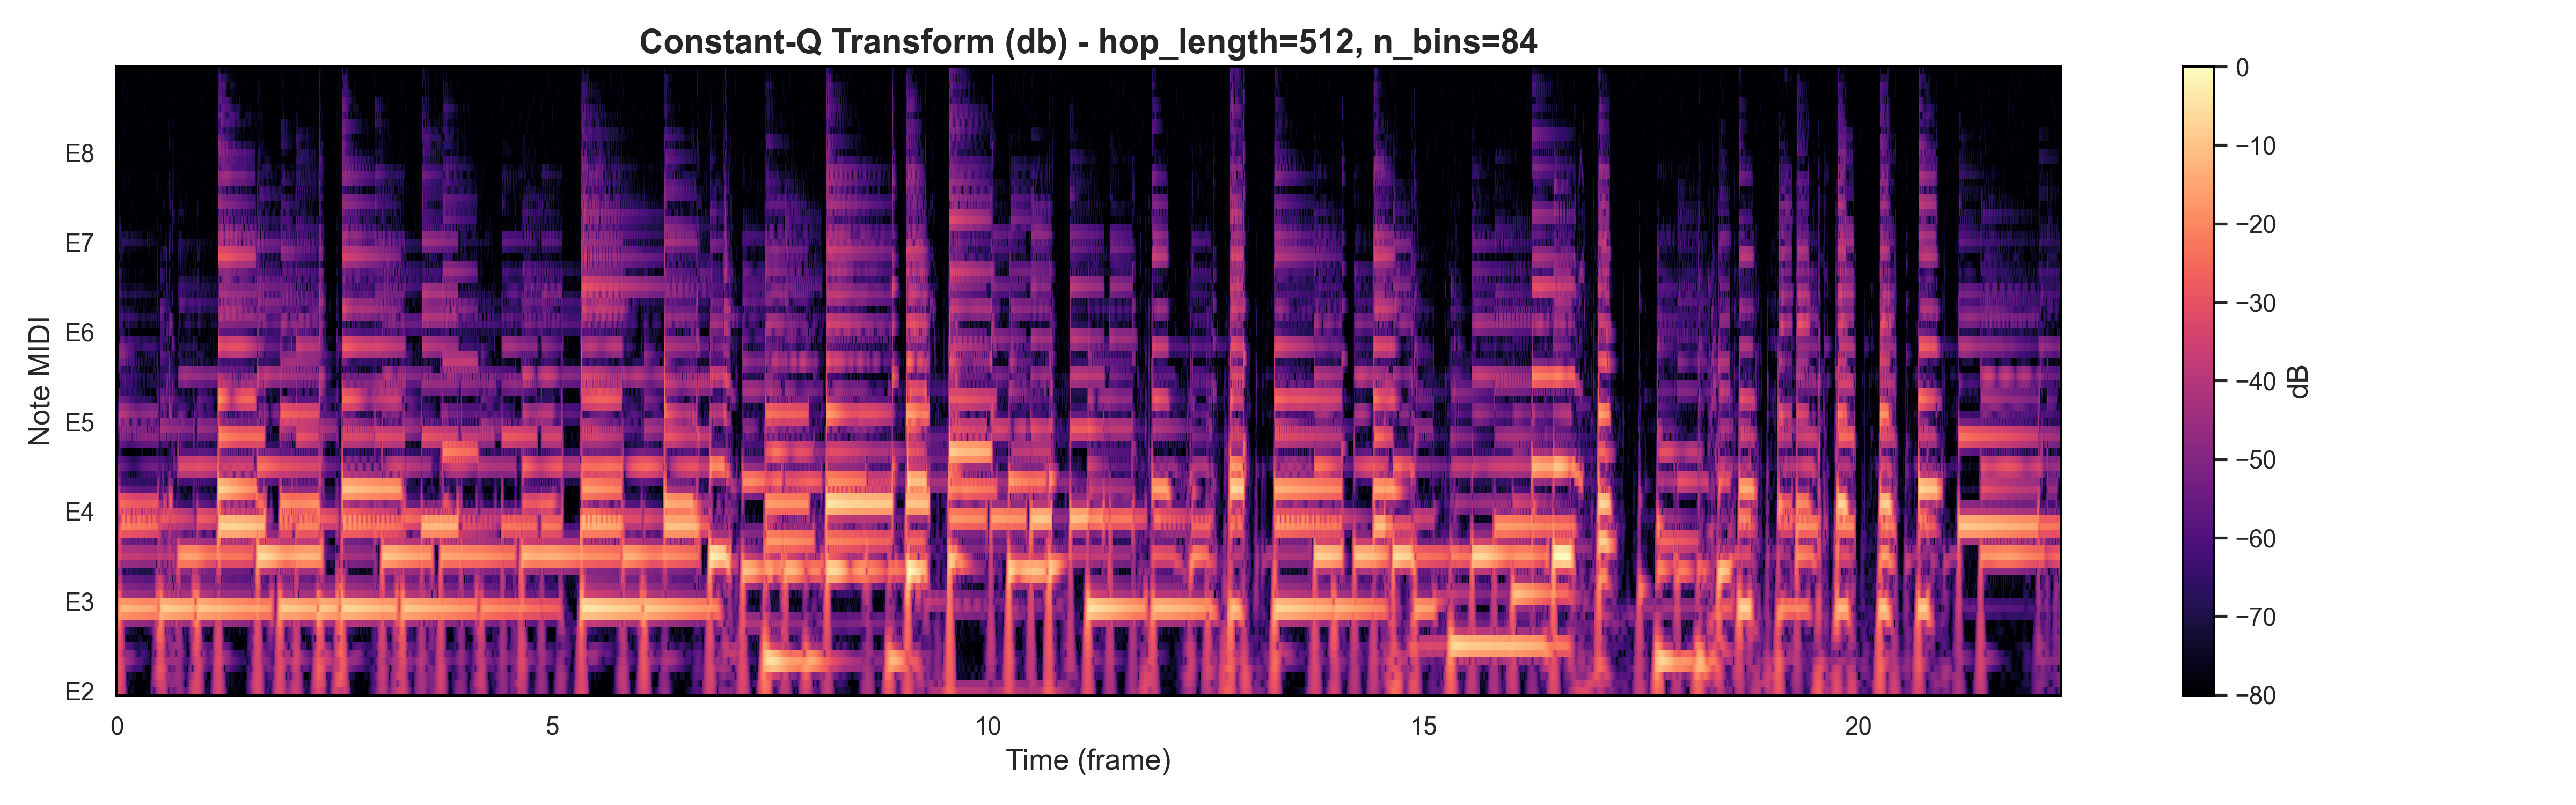
\includegraphics[height=2cm]{figures/BC02/cqt.png}
%		\end{figure}
%		
%		\small
%		La CQT est une représentation temps-fréquence adaptée à la musique. Elle fournit une représentation régulièrement utilisée en entrée des modèles d'apprentissage.
%		
%		\column{0.49\textwidth}
%		
%		\small
%		\textbf{Qualité Audio}
%		\begin{figure}
%			\centering
%			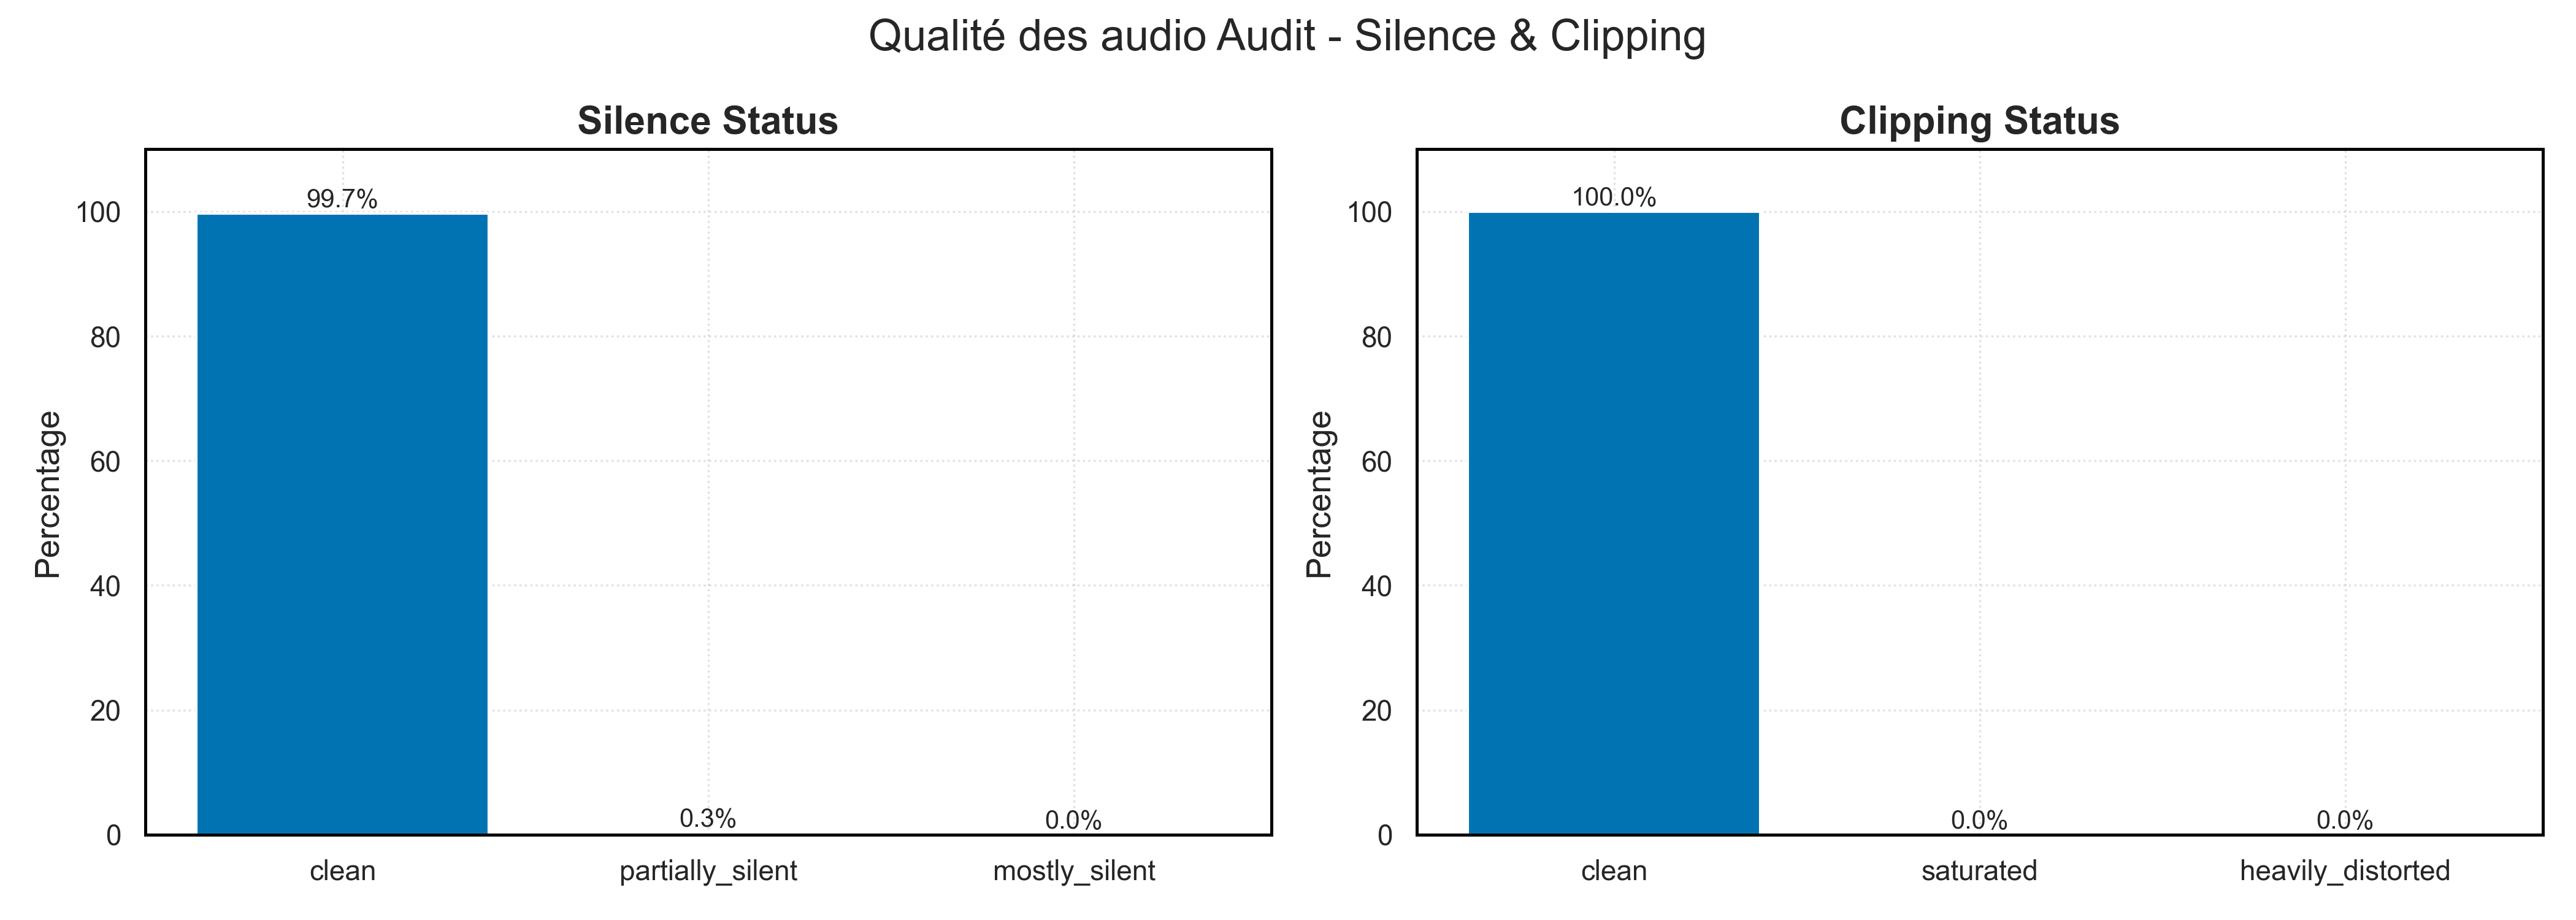
\includegraphics[width=\textwidth]{figures/BC02/audio_silence_clipping.png}
%		\end{figure}
%		
%		\small
%		Les audios sont propres, peu de silence et pas d'écrêtage.
%		
%		\vspace{0.2cm}
%		
%		\begin{block}{\small Conclusion}
%			\small
%			Dataset riche mais partiellement contraint. Bonne base pour apprentissage supervisé. IDMT-SMT-Guitar constitue un complément intéressant.
%		\end{block}
%	\end{columns}
%\end{frame}

% ===
% Analyse Dataset Frame-Wise
% ===

\begin{frame}{Analyse d'un dataset Frame-Wise - Features}
	\small
	A partir des datasets GuitarSet et IDMT-SMT-Guitar, on construis un dataset frame-wise grâce à une transformée Q-Constante (CQT).
	
	\begin{columns}[T]
		\column{0.49\textwidth}
		\begin{figure}
			\centering
			
\includegraphics[width=\textwidth]{figures/BC02/global_distribution_cqt.png}
		\end{figure}
		
		\small
		Le dataset contient énormément de bins temps-fréquence sans énergie, cela implique un fort déséquilibre des données. Le modèle risque de ne pas détecter l'activation des notes. Il faudra privilégier une standardisation robuste : $x' = \dfrac{x - \text{médiane}}{IQR}$.
		
		\column{0.49\textwidth}
		
		\small
		
		\begin{figure}
			\centering
			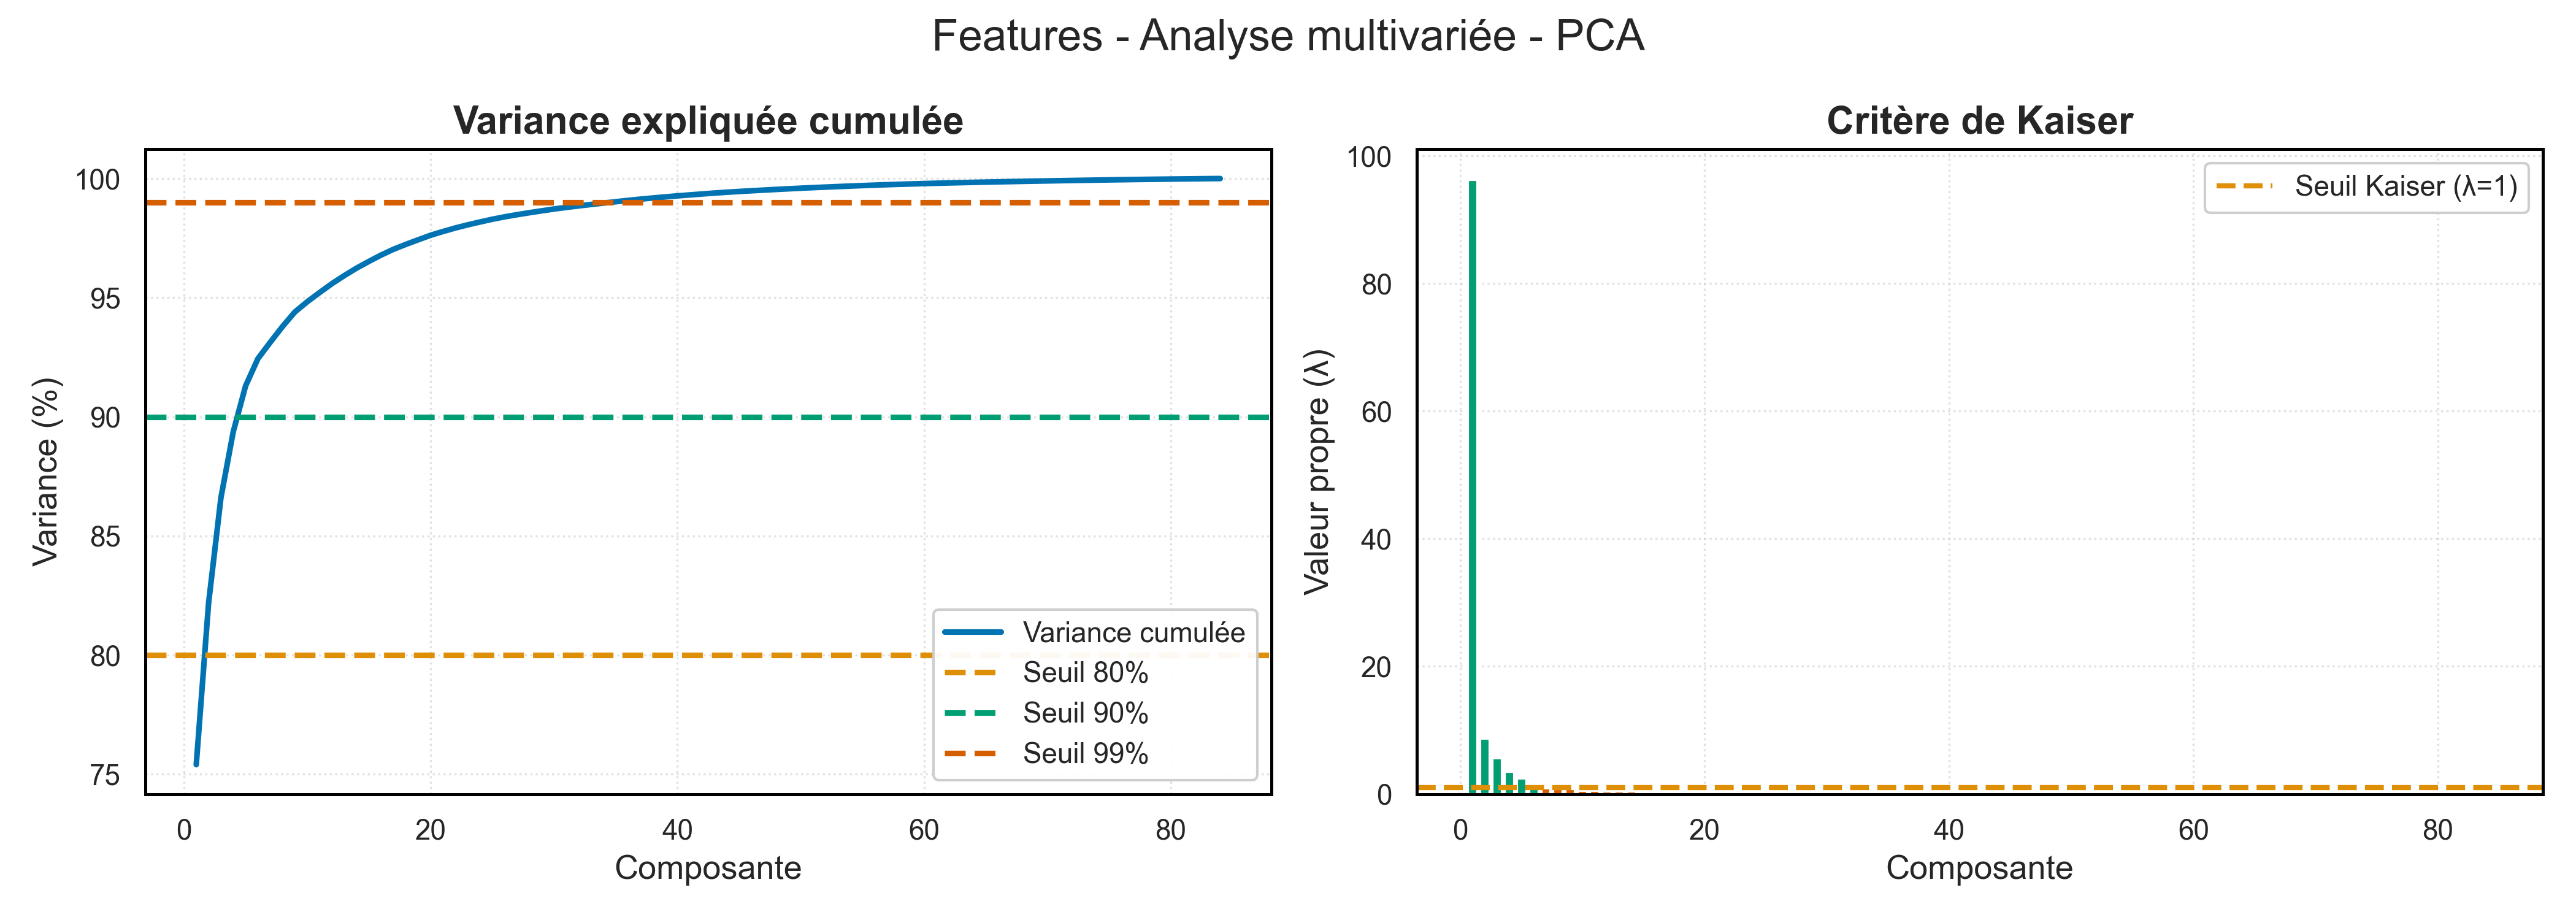
\includegraphics[width=\textwidth]{figures/BC02/pca.png}
		\end{figure}
		
		\small
		L'analyse des corrélations entre features permet d'envisager une PCA. 6 valeurs propres supérieures à 1. Elles expliquent au moins 92\% de la variance.
	\end{columns}
\end{frame}

\begin{frame}{Analyse d'un dataset Frame-Wise - Target}
	\vspace{-0.2cm}
	
	\begin{columns}[T]
		\column{0.49\textwidth}
		
		\begin{figure}
			\centering
			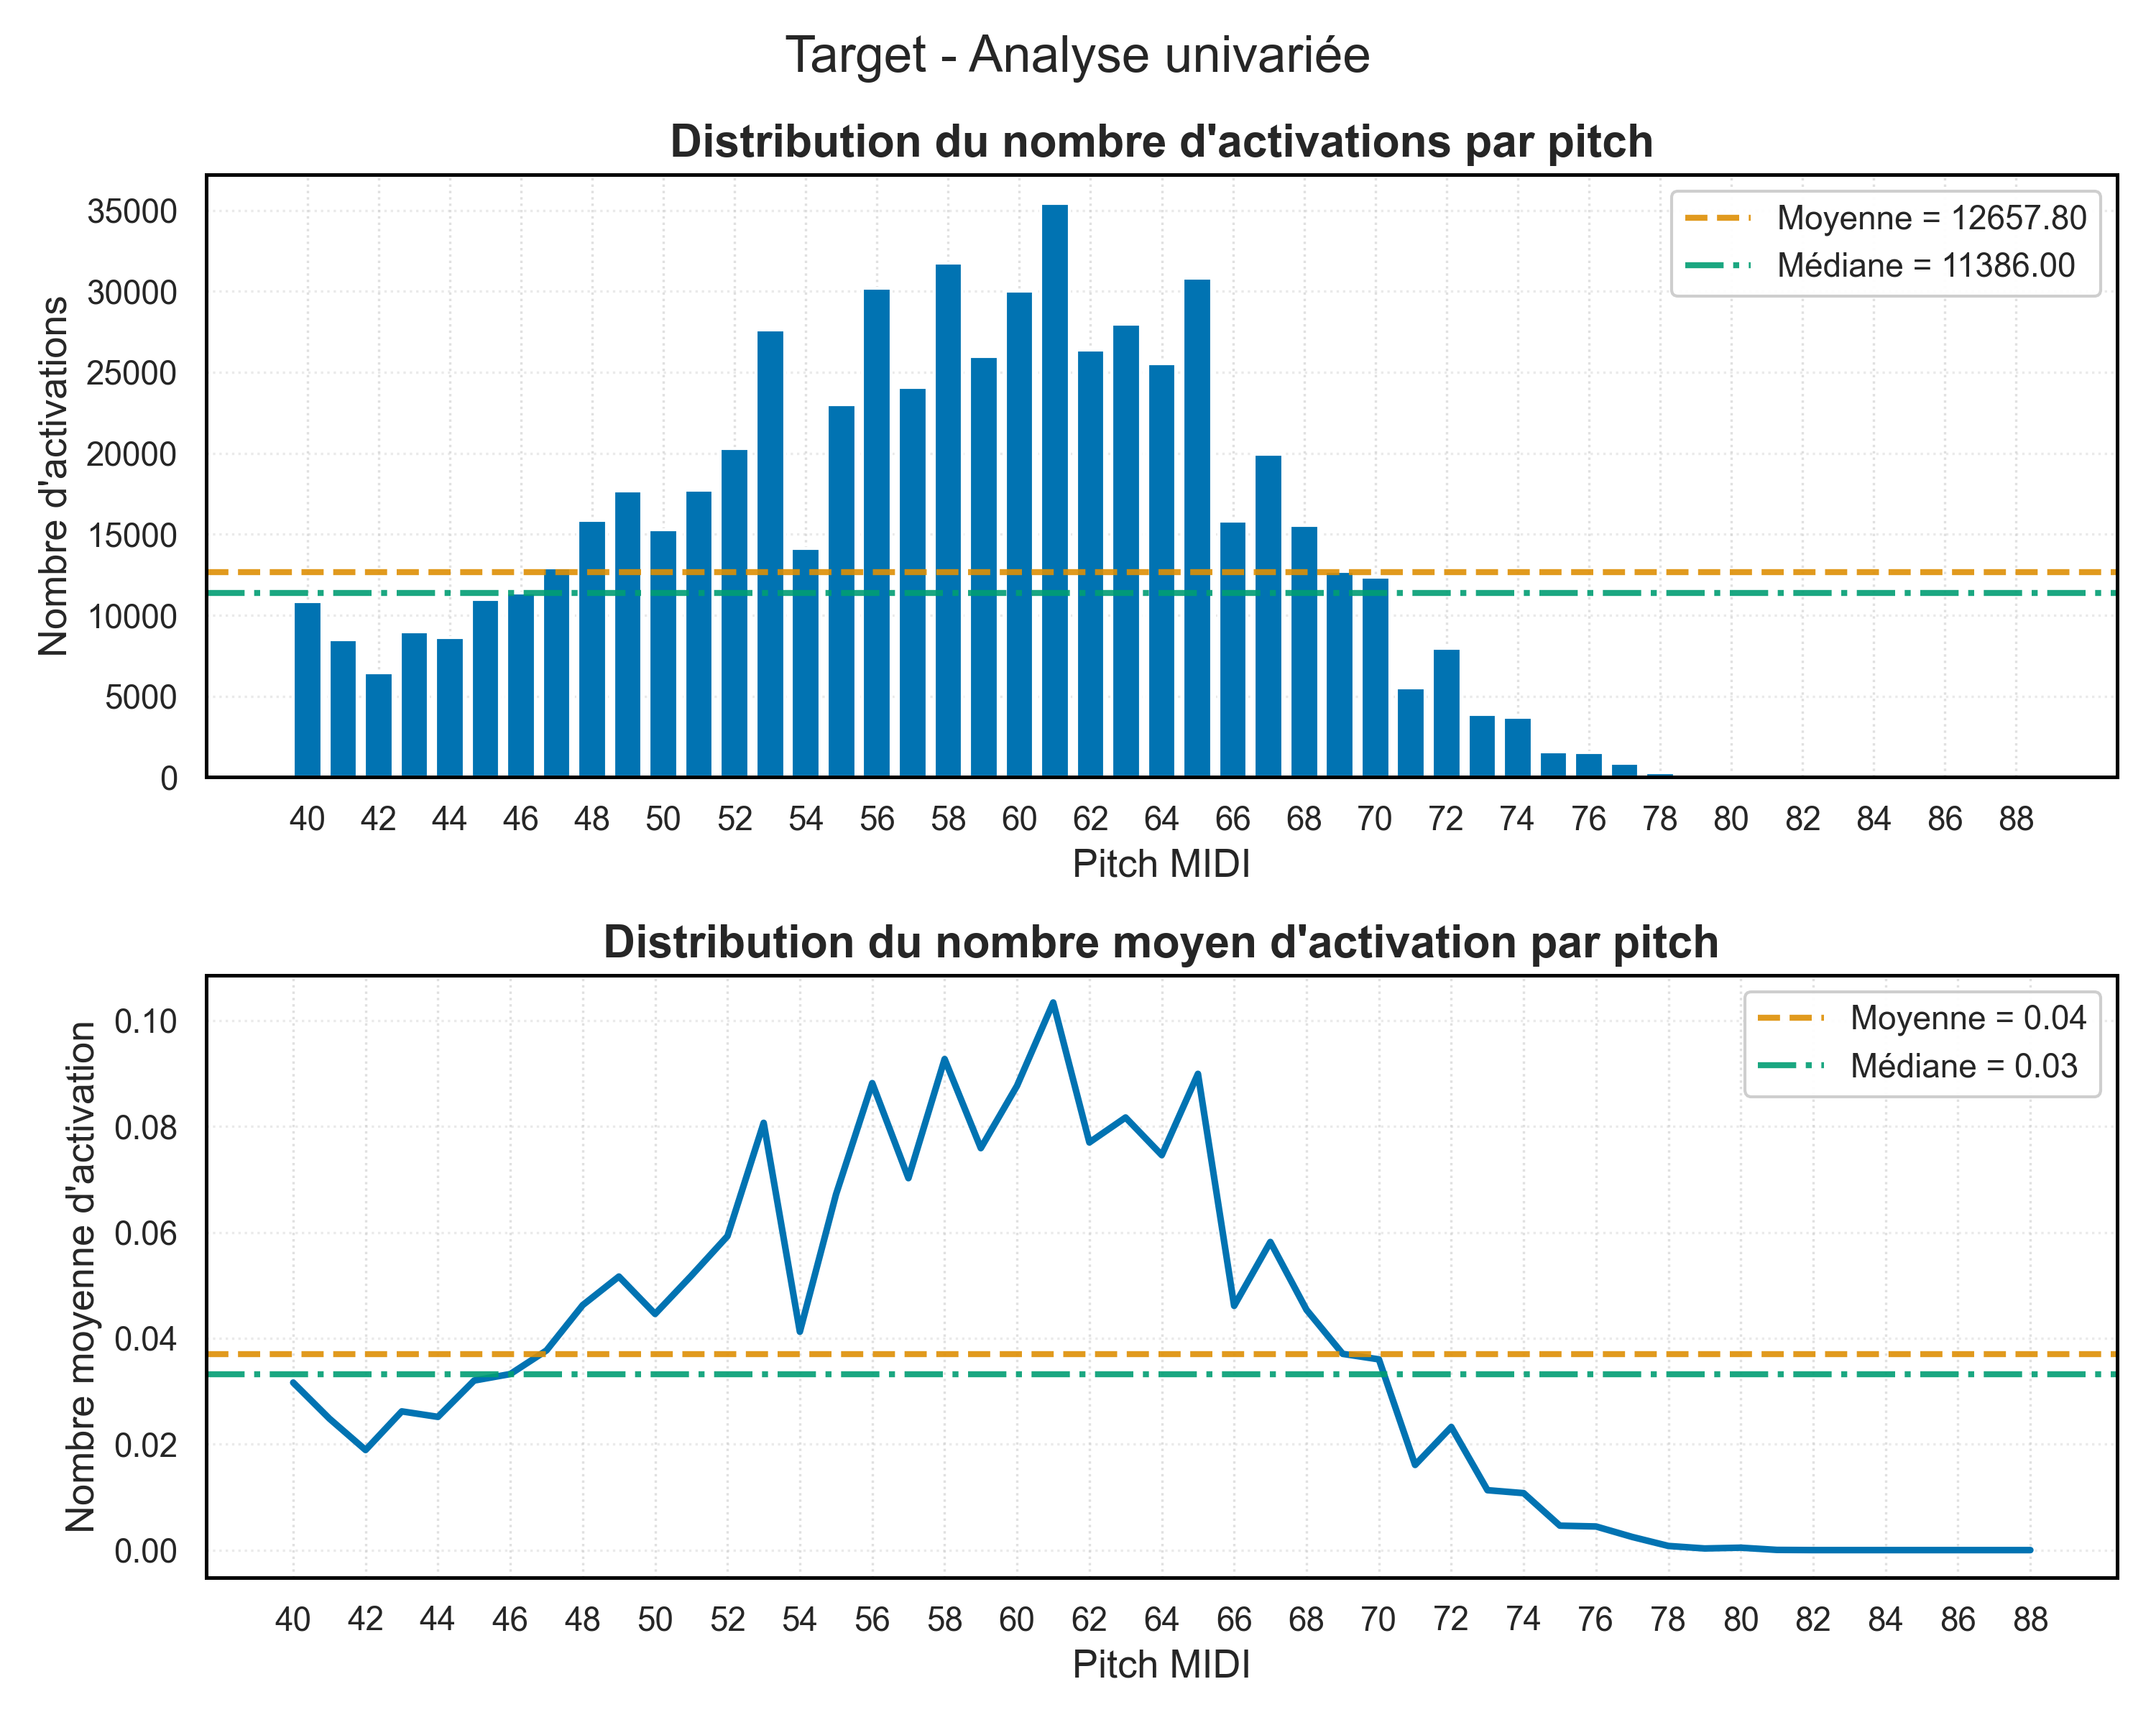
\includegraphics[height=5cm]{figures/BC02/activation_pitch_analysis.png}
		\end{figure}
		
		\small
		Le déséquilibre des classes est un réel problème, le modèle risque de ne pas détecter d'activation. La distribution des activations de notes est hétérogène, les notes aiguës seront plus difficiles à détecter.
		
		\column{0.49\textwidth}
		
		\begin{figure}
			\centering
			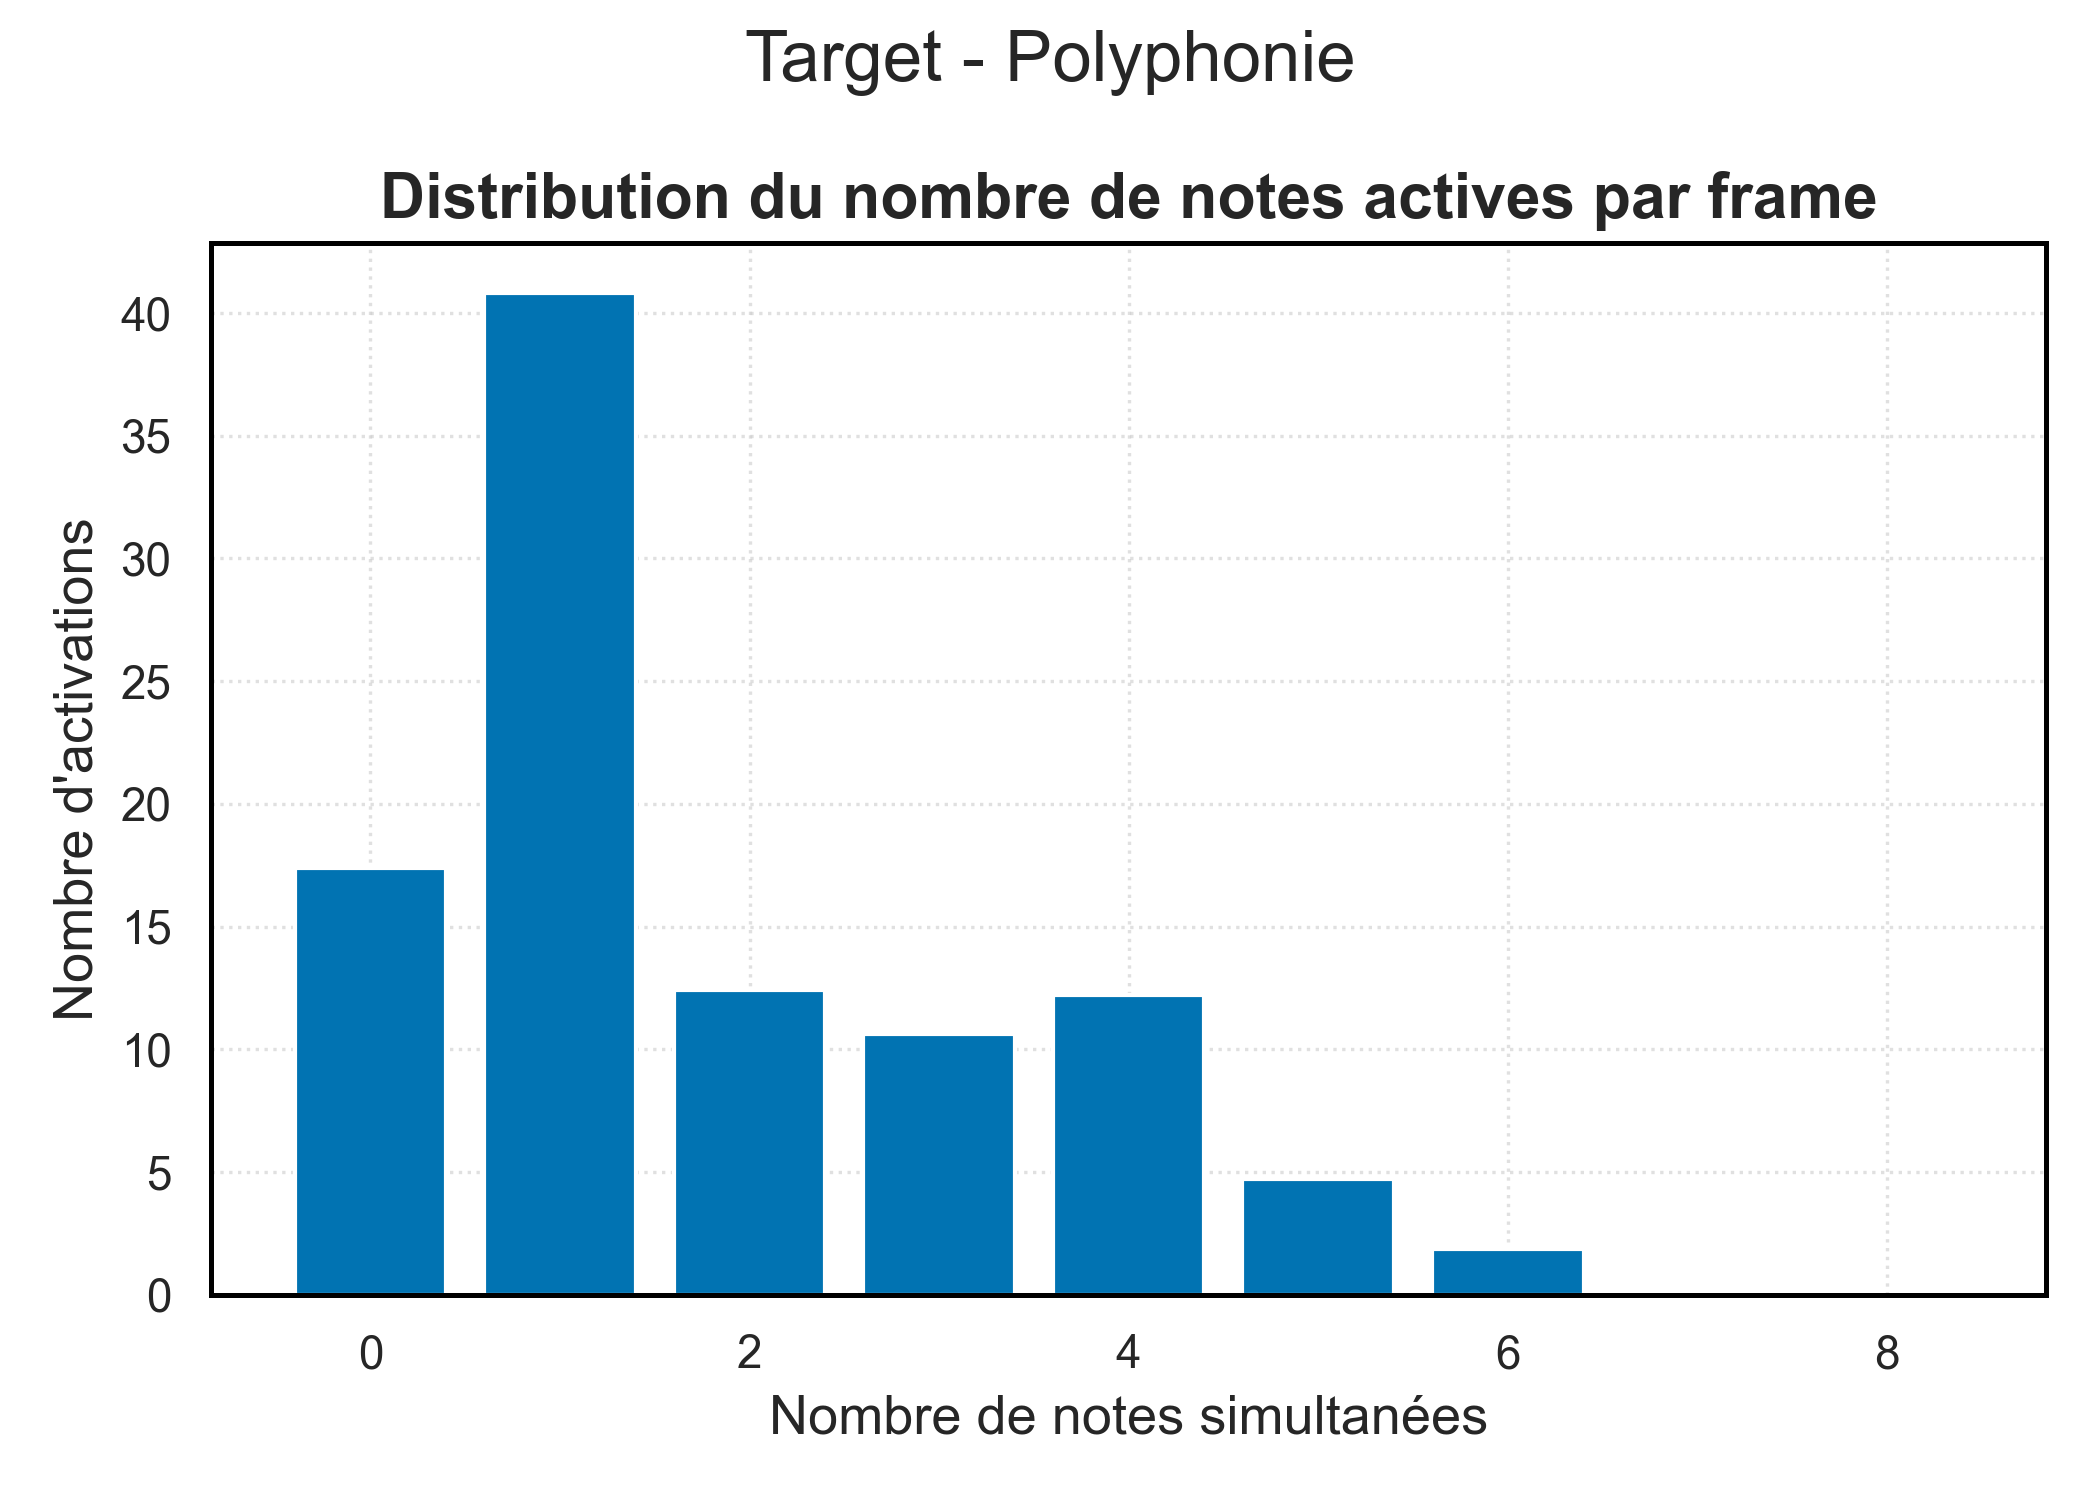
\includegraphics[height=3cm]{figures/BC02/distibution_simultaneous_activations.png}
		\end{figure}
		
		\small
		63 frames contiennent plus de 6 activations simultanées, non aligné avec la physique de l'instrument.
	\end{columns}
\end{frame}